\documentclass[12pt]{article}
\usepackage[margin=0.8in]{geometry}
\usepackage[utf8]{inputenc}
\usepackage{graphicx}
\usepackage[export]{adjustbox}
\graphicspath{ {../Images/} }
\usepackage{amsmath}
\usepackage{amsfonts}
\usepackage{amssymb}
\usepackage[version=4]{mhchem}
\usepackage{stmaryrd}
\usepackage{bbold}
%\usepackage[fallback]{xeCJK}
\usepackage{polyglossia}
\usepackage{fontspec}
%\setCJKmainfont{Noto Serif CJK TC}

\usepackage{tikz}
\usepackage{amsthm}
\usepackage{tcolorbox}
\usepackage{enumitem}% http://ctan.org/pkg/enumitem

\tcbuselibrary{theorems}

\definecolor{GrayBG}{HTML}{d9d9d9}
\definecolor{BlueDef}{HTML}{104e8b}
\definecolor{GreenProp}{HTML}{025540}
\definecolor{RedMet}{HTML}{cd5556}
\definecolor{BrownHist}{HTML}{8b5a2b}
\definecolor{BlackSav}{HTML}{000000}

\newcommand{\hideM}[1]{\mbox{\vphantom{$#1$}\smash{\colorbox{gray!50}{$\displaystyle #1$}}} }
\newcommand{\hide}[1]{\mbox{\vphantom{#1}\smash{\colorbox{gray!50}{#1}}}}
%\newcommand{\hideM}[1]{\mbox{\vphantom{$#1$}\smash{\colorbox{gray!50}{\phantom{$\displaystyle #1$}}}} }
%\newcommand{\hide}[1]{\mbox{\vphantom{#1}\smash{\colorbox{gray!50}{\phantom{#1}}}}}

\newtcbtheorem
  []% init options
  {definition}% name
  {Définition}% title
  {%
    colback=GrayBG,
    colframe=BlueDef,
    fonttitle=\bfseries,
  }% options
  {def}% prefix

\newtcbtheorem
  []% init options
  {proposition}% name
  {Proposition}% title
  {%
    colback=GrayBG,
    colframe=GreenProp,
    fonttitle=\bfseries,
  }% options
  {prop}% prefix

\newtcbtheorem
  []% init options
  {method}% name
  {Méthode}% title
  {%
    theorem name,
    colback=GrayBG,
    colframe=RedMet,
    fonttitle=\bfseries,
  }% options
  {met}% prefix
  
\newtcbtheorem
  []% init options
  {history}% name
  {Histoire}% title
  {%
    theorem name,
    colback=GrayBG,
    colframe=BrownHist,
    fonttitle=\bfseries,
  }% options
  {hist}% prefix
  
\newtcbtheorem
  []% init options
  {savoir}% name
  {Savoir-faire du chapitre}% title
  {%
    theorem name,
    colback=GrayBG,
    colframe=BlackSav,
    fonttitle=\bfseries,
  }% options
  {sav}% prefix

\newtheoremstyle{break}
  {}
  {}
  {}
  {}
  {\bfseries}
  {}
  {\newline}
  {}
\theoremstyle{break}
\newtheorem*{example}{Exemple.}
\newtheorem*{examples}{Exemples.}
\newtheorem*{remark}{Remarque.}

\newenvironment{demo}[1][\proofname]{%
  \begin{proof}[#1]$ $\newline
}{%
  \end{proof}
}

\setmainlanguage{french}
%\setmainf[tikznode]ont{CMU Serif}

\title{
\vspace{4em}
\centering
\tcbset{colframe=BlackSav,colback=GrayBG}
\tcbox[tikznode]{
Chapitre 7 \\ Matrices et systèmes linéaires
}
}

\author{}
\date{}

\setlength\parindent{0pt}

\begin{document}
\maketitle

\tableofcontents

\newpage


\section*{Introduction}
Résoudre le système d'équations suivant :

$$
\left\{\begin{array}{r}
x_{2}-x_{3}=4 \\
2 x_{1}+2 x_{2}-3 x_{3}=8 \\
4 x_{1}+x_{2}+x_{3}=8
\end{array}\right.
$$

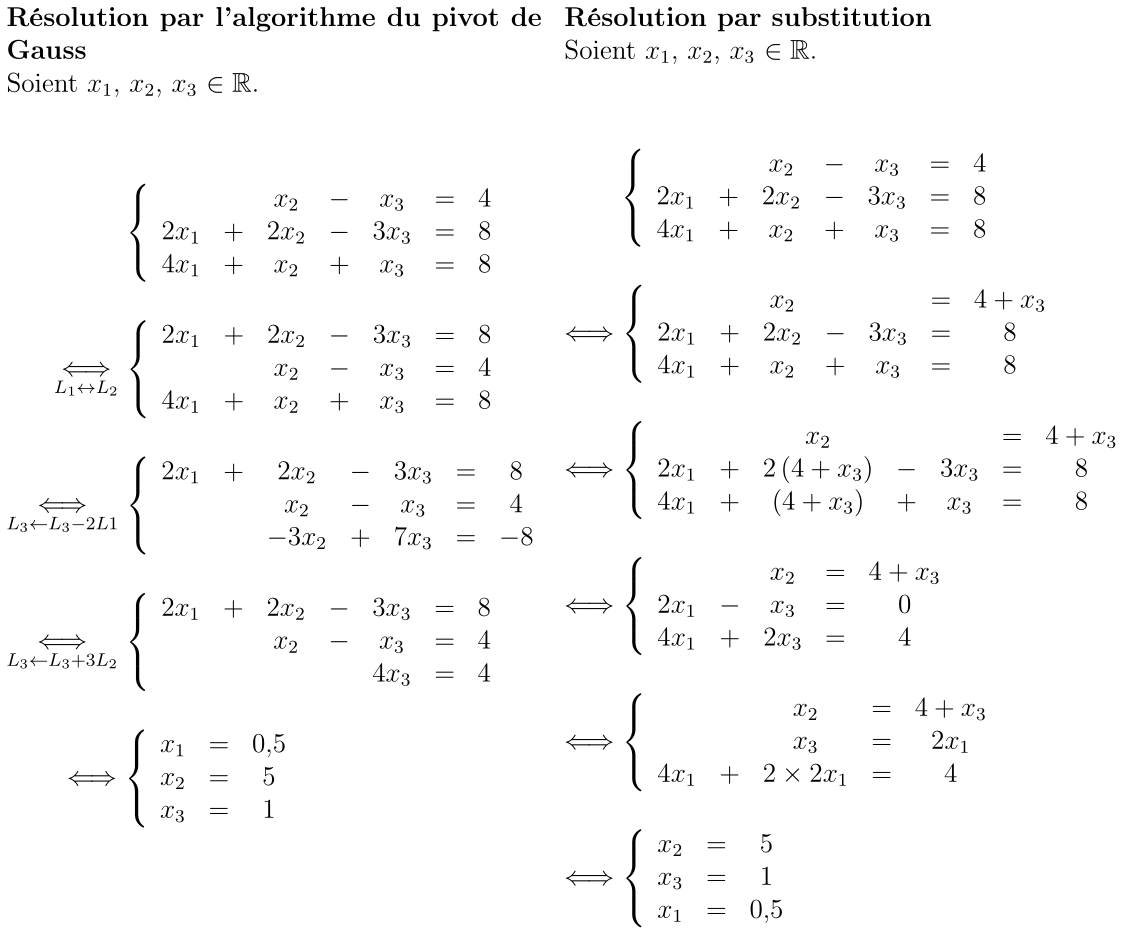
\includegraphics[width=1\textwidth]{swappy-20250331_122603.png}

\begin{method}{Algorithme du pivot de Gauss pour résoudre un système}{}
On effectue des opérations sur les lignes consistant à :

\begin{itemize}[noitemsep,topsep=0pt]
  \item Permuter entre elles deux lignes du système pour faire apparaître un nombre non nul dans le coin supérieur gauche (le pivot)
  \item Multiplier une ligne du système par un nombre non nul.
  \item Faire une opération de la forme $L_{i} \longleftarrow L_{i}-\lambda L_{j}$ (transvection) afin de faire apparaître un 0 .
\end{itemize}
\end{method}

\newpage
\begin{remark}
L'avantage de la méthode du pivot de Gauss réside dans le fait que les calculs se mènent indépendamment sur la partie gauche et la partie droite des égalités. Ainsi, si l'on souhaite par exemple résoudre le système $\left\{\begin{aligned} & x_{2}-x_{3}=4 \\ & 2 x_{1}+2 x_{2}-3 x_{3}=8 \\ & 4 x_{1}+x_{2}+x_{3}=8\end{aligned}\right.$, les calculs à gauche des signes «égal» resteront les mêmes. Cela n'est en revanche pas le cas dans la méthode de résolution par substitution. Pour cette raison, on privilégiera donc la méthode du pivot de Gauss.

De plus, le fait que les calculs se font indépendamment à gauche et à droite des signes «égal» permet, pour ainsi dire, de ne s'intéresser qu'à la partie de gauche. On omet même de noter les variables et on résume les coefficients du système dans un tableau, appelé matrice. Pour le système résolu ci-dessus, la matrice associée au système est

$$
\left(\begin{array}{ccc}
0 & 1 & -1 \\
2 & 2 & -3 \\
4 & 1 & 1
\end{array}\right)
$$
\end{remark}

\noindent
\begin{minipage}{.7\textwidth}
  \begin{history}{Matrices}{}
    Si le terme «matrice» date du XIX$^{e}$ siècle, l'idée de former un tableau des coefficients pour résoudre un système d'équations linéaires est en revanche beaucoup plus ancienne. Ainsi, le texte chinois intitulé Les Neuf Chapitres sur l'art mathématique, écrit vers le $I^{\mathrm{e}}$ siècle av. J.-C., contient des tableaux permettant de résoudre des systèmes d'équations. Ces mêmes idées seront bien plus tard à l'origine de la théorie des matrices. Notons enfin qu'au XIX ${ }^{\text {e }}$ siècle, beaucoup de propriétés sur les matrices seront démontrées d'abord sur des matrices à 2 ou 3 lignes et colonnes avant d'être généralisées dans le cas général.
  \end{history}
\end{minipage}
\hspace{1em}
\begin{minipage}{0.35\textwidth}
  \begin{tcolorbox}[colback=white,colframe=BrownHist]
    \centering
    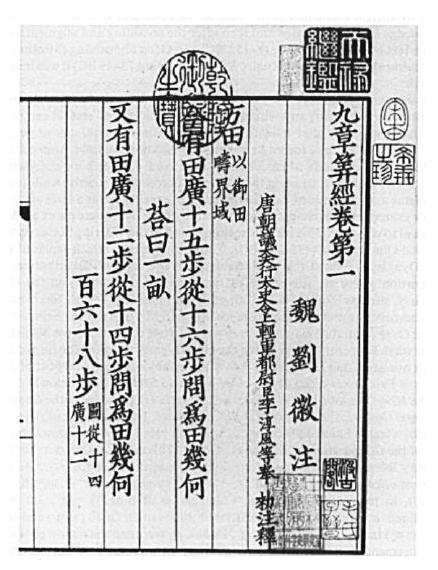
\includegraphics[max width=\textwidth, center]{2025_03_28_69fb641a049744196071g-03}
    Les Neuf Chapitres sur l'art mathématique
  \end{tcolorbox}
\end{minipage}

\newpage

\section{Matrices : définitions et premières propriétés}
\subsection{Définitions}
Dans tout le chapitre, $\mathbb{K}$ désigne l'ensemble $\mathbb{R}$ ou $\mathbb{C}$.

\begin{definition}{}{}
\begin{itemize}[noitemsep,topsep=0pt]
  \item Une \hide{matrice} à coefficients dans $\mathbb{K}$ et de taille $n \times m$ est un tableau de nombres appartenant à $\mathbb{K}$ et possédant $n$ lignes et $m$ colonnes.
  \item L'ensemble des matrices à coefficients dans $\mathbb{K}$ et de taille $n \times m$ est noté $\hideM{\mathcal{M}_{n, m}(\mathbb{K})}$.
\end{itemize}
\end{definition}

\begin{example}
La matrice $\left(\begin{array}{ccc}1 & \sqrt{2} & 0 \\ -6 & 0 & 9\end{array}\right)$ est une matrice de taille $2 \times 3$ à coefficients dans $\mathbb{R}$.
\end{example}

\begin{remark}
En général, on note $\left(a_{i, j}\right)$ avec $1 \leqslant i \leqslant n$ et $1 \leqslant j \leqslant m$ la matrice à $n$ lignes et $m$ colonnes, où $a_{i, j}$ désigne le coefficient situé à la ie ligne et $\mathrm{j}^{\mathrm{e}}$ colonne. On utilise parfois aussi la notation suivante:

$$
\left(\begin{array}{ccccc}
a_{1,1} & \ldots & a_{1, j} & \ldots & a_{1, m} \\
\vdots & & \vdots & & \vdots \\
a_{i, 1} & \ldots & a_{i, j} & \ldots & a_{i, m} \\
\vdots & & \vdots & & \vdots \\
a_{n, 1} & \ldots & a_{n, j} & \ldots & a_{n, m}
\end{array}\right)
$$
\end{remark}

\begin{definition}{}{}
Soit M une matrice.

\begin{itemize}[noitemsep,topsep=0pt]
  \item Lorsque $n=1$, on dit que M est une \textbf{matrice ligne}.
  \item Lorsque $m=1$, on dit que M est une \textbf{matrice colonne}.
  \item Lorsque $n=m$, on dit que M est une \textbf{matrice carrée} d'ordre $n$.
  \item Lorsque $n=m$ et que pour tout $i \neq j, a_{i, j}=0$, on dit que M est une \textbf{matrice diagonale}.
  \item La \textbf{matrice identité} d'ordre $n$ est la matrice diagonale de taille $n \times n$ dont tous les coefficients diagonaux sont égaux à 1 . On la note $\mathrm{I}_{n}$.
  \item La \textbf{matrice nulle} de taille $n \times m$ est la matrice de taille $n \times m$, dont tous les coefficients sont nuls. On la note $0_{n \times m}$.
\end{itemize}
\end{definition}

\begin{definition}{}{}
Deux matrices A et B sont \textbf{égales} si et seulement si elles sont de même \hide{tailles} et ont les mêmes \hide{coefficients}.
\end{definition}

\newpage
\begin{definition}{}{}
Une matrice carrée $\mathrm{A}=\left(a_{i, j}\right)$ est dite \textbf{symétrique} lorsque pour tous $i$ et $j, \hideM{a_{i, j}=a_{j, i}}$.
\end{definition}

\begin{example}
La matrice $\left(\begin{array}{ccc}1 & \sqrt{2} & 4 \\ \sqrt{2} & 0 & -8 \\ 4 & -8 & 7\end{array}\right)$ est une matrice symétrique.
\end{example}

\subsection{Somme de matrices et multiplication d'une matrice par un scalaire}
\begin{definition}{}{}
Soient $\mathrm{A}=\left(a_{i, j}\right)$ et $\mathrm{B}=\left(b_{i, j}\right)$ deux matrices de taille $n \times m$.

\begin{itemize}[noitemsep,topsep=0pt]
  \item La \textbf{somme des matrices} A et B , notée $A+B$, est la matrice $\mathrm{C}=\left(c_{i, j}\right)$ de taille $n \times m$ telle que, pour tous $1 \leqslant i \leqslant n$ et $1 \leqslant j \leqslant m$, on a $c_{i, j}=\hideM{a_{i, j}+b_{i, j}}$.
  \item Le \textbf{produit de la matrice A par $\lambda \in \mathbb{K}$}, noté $\lambda \mathrm{A}$, est la matrice $\mathrm{M}=\left(m_{i, j}\right)$ de taille $n \times m$ telle que, pour tous $1 \leqslant i \leqslant n$ et $1 \leqslant j \leqslant m$, on a $m_{i, j}=\hideM{\lambda \times a_{i, j}}$.
\end{itemize}
\end{definition}

\begin{example}
Si $A=\left(\begin{array}{cc}1 & 2 \\ -4 & 3\end{array}\right)$ et $B=\left(\begin{array}{ll}5 & 0 \\ 1 & 3\end{array}\right)$.\\
On a alors $A+B=\left(\begin{array}{cc}6 & 2 \\ -3 & 6\end{array}\right)$.\\
et $3 \mathrm{~A}=\left(\begin{array}{cc}3 & 6 \\ -12 & 9\end{array}\right)$.
\end{example}

\begin{proposition}{}{}
Soient $\mathrm{A}, \mathrm{B}$ et C trois matrices de même taille et $\alpha, \beta \in \mathbb{K}$.
\begin{itemize}[noitemsep,topsep=0pt]
  \item $A+B=B+A$ (commutativité de la somme de matrices)
  \item $(\mathrm{A}+\mathrm{B})+\mathrm{C}=\mathrm{A}+(\mathrm{B}+\mathrm{C})$ (associativité de la somme de matrices)
  \item $(\mathrm{A}+\mathrm{B})+\mathrm{C}=\mathrm{A}+(\mathrm{B}+\mathrm{C}) \quad$ (associativité de la somme de matrices)
  \item $1 \times \mathrm{A}=\mathrm{A}$.
  \item $(\alpha+\beta) \mathrm{A}=\alpha \mathrm{A}+\beta \mathrm{A}$
  \item $\alpha(\mathrm{A}+\mathrm{B})=\alpha \mathrm{A}+\beta \mathrm{B}$
\end{itemize}
\end{proposition}

\begin{definition}{}{}
\begin{itemize}[noitemsep,topsep=0pt]
  \item On appelle \textbf{opposé} de A la matrice $\hideM{(-1) \times \mathrm{A}}$. On la note -A .
  \item On note $\mathrm{A}-\mathrm{B}$ la matrice $\mathrm{A}+(-\mathrm{B})$.
\end{itemize}
\end{definition}

\newpage
\section{Applications linéaires et matrices}
Dans toute la suite, et par abus de notation, on identifiera un vecteur $\vec{v}$ avec ses coordonnées. Par exemple, pour un vecteur $\vec{v}\left(\begin{array}{l}a \\ b \\ c\end{array}\right)$ et une application $f: \mathbb{R}^{3} \longrightarrow \mathbb{R}^{3}$, on notera indifféremment $f(a ; b ; c)$ ou $f(\vec{v})$ l'image de $(a ; b ; c)$ par $f$.

\subsection{Applications linéaires}
\begin{definition}{}{}
Soient $n$ et $m$ deux entiers naturels non nuls. On considère une application $f: \mathbb{K}^{m} \longrightarrow$ $\mathbb{K}^{n}$.\\
On dit que $f$ est linéaire si pour tous $\vec{u}, \vec{v} \in \mathbb{K}^{m}$ et $\lambda \in \mathbb{K}$ :

$$
\left\{\begin{array}{l}
f(\vec{u}+\vec{v})=\hideM{f(\vec{u})+f(\vec{v})} \\
\text { et } \\
f(\lambda \vec{u})=\hideM{\lambda f(\vec{u})}
\end{array}\right.
$$
\end{definition}

\begin{definition}{}{}
L'ensemble des applications linéaires de $\mathbb{K}^{m}$ dans $\mathbb{K}^{n}$ est noté $\mathcal{L}\left(\mathbb{K}^{m}, \mathbb{K}^{n}\right)$.
\end{definition}

\begin{proposition}{}{}
La composée de deux applications linéaires est une application linéaire.
\end{proposition}

\begin{demo}
Voir exercice.
\end{demo}

\begin{definition}{ - (Propriété/Définition)}{}
Soient $n$ et $m$ deux entiers naturels non nuls.\\
Une application $f: \mathbb{K}^{m} \longrightarrow \mathbb{K}^{n}$ est linéaire si, et seulement si, il existe $\left(a_{i, j}\right) \in \mathcal{M}_{n, m}(\mathbb{K})$ telle que, pour tout $\left(x_{1}, x_{2}, \ldots, x_{m}\right) \in \mathbb{K}^{m}$,

$$
f\left(x_{1}, x_{2}, \ldots, x_{m}\right)=\left(\begin{array}{c}
a_{1,1} x_{1}+a_{1,2} x_{2}+\ldots+a_{1, m} x_{m} \\
a_{2,1} x_{1}+a_{2,2} x_{2}+\ldots+a_{2, m} x_{m} \\
\ldots \\
\ldots \\
a_{n, 1} x_{1}+a_{n, 2} x_{2}+\ldots+a_{n, m} x_{m}
\end{array}\right)
$$

On dit que la matrice $\mathrm{A}=\left(a_{i, j}\right)$ est la \textbf{matrice associée} à $f$ et on note

$$
\hideM{\operatorname{Mat}(f)}=\mathrm{A}
$$
\end{definition}

\newpage
\begin{demo}
Soit $f: \mathbb{K}^{m} \longrightarrow \mathbb{K}^{n}$.

\begin{itemize}[noitemsep,topsep=0pt]
  \item Supposons qu'il existe $\left(a_{i, j}\right) \in \mathcal{M}_{n, m}(\mathbb{K})$ telle que, pour tout $\left(x_{1}, x_{2}, \ldots, x_{m}\right) \in \mathbb{K}^{m}$,
\end{itemize}

$$
f\left(x_{1}, x_{2}, \ldots, x_{m}\right)=\left(\begin{array}{c}
a_{1,1} x_{1}+a_{1,2} x_{2}+\ldots+a_{1, m} x_{m} \\
a_{2,1} x_{1}+a_{2,2} x_{2}+\ldots+a_{2, m} x_{m} \\
\ldots \\
\ldots \\
a_{n, 1} x_{1}+a_{n, 2} x_{2}+\ldots+a_{n, m} x_{m}
\end{array}\right) .
$$

On va montrer que $f$ est linéaire.\\
Soient $\vec{u}\left(x_{1} ; x_{2} ; \ldots ; x_{m}\right) \in \mathbb{K}^{m}$ et $\vec{v}\left(y_{1} ; y_{2} ; \ldots ; y_{m}\right) \in \mathbb{K}^{m}$ deux vecteurs et soit $\lambda \in \mathbb{K}$.\\
D'une part,

$$
\begin{aligned}
f(\vec{u})+f(\vec{v}) & =f\left(x_{1}, x_{2}, \ldots, x_{m}\right)+f\left(y_{1}, y_{2}, \ldots, y_{m}\right) \\
& =\left(\begin{array}{c}
a_{1,1} x_{1}+a_{1,2} x_{2}+\ldots+a_{1, m} x_{m} \\
a_{2,1} x_{1}+a_{2,2} x_{2}+\ldots+a_{2, m} x_{m} \\
\ldots \\
\ldots \\
a_{n, 1} x_{1}+a_{n, 2} x_{2}+\ldots+a_{n, m} x_{m}
\end{array}\right)+\left(\begin{array}{c}
a_{1,1} y_{1}+a_{1,2} y_{2}+\ldots+a_{1, m} y_{m} \\
a_{2,1} y_{1}+a_{2,2} y_{2}+\ldots+a_{2, m} y_{m} \\
\ldots \\
\ldots \\
a_{n, 1} y_{1}+a_{n, 2} y_{2}+\ldots+a_{n, m} y_{m}
\end{array}\right) \\
& =\left(\begin{array}{c}
\left(a_{1,1} x_{1}+a_{1,2} x_{2}+\ldots+a_{1, m} x_{m}\right)+\left(a_{1,1} y_{1}+a_{1,2} y_{2}+\ldots+a_{1, m} y_{m}\right) \\
\left(a_{2,1} x_{1}+a_{2,2} x_{2}+\ldots+a_{2, m} x_{m}\right)+\left(a_{2,1} y_{1}+a_{2,2} y_{2}+\ldots+a_{2, m} y_{m}\right) \\
\ldots \\
\ldots \\
\left(a_{n, 1} x_{1}+a_{n, 2} x_{2}+\ldots+a_{n, m} x_{m}\right)+\left(a_{n, 1} y_{1}+a_{n, 2} y_{2}+\ldots+a_{n, m} y_{m}\right)
\end{array}\right) \\
& =\left(\begin{array}{c}
a_{1,1}\left(x_{1}+y_{1}\right)+a_{1,2}\left(x_{2}+y_{2}\right)+\ldots+a_{1, m}\left(x_{m}+y_{m}\right) \\
a_{2,1}\left(x_{1}+y_{1}\right)+a_{2,2}\left(x_{2}+y_{2}\right)+\ldots+a_{2, m}\left(x_{m}+y_{m}\right) \\
\ldots \\
\ldots \\
a_{n, 1}\left(x_{1}+y_{1}\right)+a_{n, 2}\left(x_{2}+y_{2}\right)+\ldots+a_{n, m}\left(x_{m}+y_{m}\right)
\end{array}\right) \\
& =f(\vec{u}+\vec{v})
\end{aligned}
$$

D'autre part,

$$
\begin{aligned}
f(\lambda \vec{u}) & =f\left(\lambda x_{1} ; \lambda x_{2} ; \ldots ; \lambda x_{m}\right) \\
& =\left(\begin{array}{c}
a_{1,1} \lambda x_{1}+a_{1,2} \lambda x_{2}+\ldots+a_{1, m} \lambda x_{m} \\
a_{2,1} \lambda x_{1}+a_{2,2} \lambda x_{2}+\ldots+a_{2, m} \lambda x_{m} \\
\ldots \\
\ldots \\
a_{n, 1} \lambda x_{1}+a_{n, 2} \lambda x_{2}+\ldots+a_{n, m} \lambda x_{m}
\end{array}\right) \\
& =\lambda\left(\begin{array}{c}
a_{1,1} x_{1}+a_{1,2} x_{2}+\ldots+a_{1, m} x_{m} \\
a_{2,1} x_{1}+a_{2,2} x_{2}+\ldots+a_{2, m} x_{m} \\
\ldots \\
\ldots \\
a_{n, 1} x_{1}+a_{n, 2} x_{2}+\ldots+a_{n, m} x_{m}
\end{array}\right) \\
& =\lambda f(\vec{u})
\end{aligned}
$$

Ainsi, on a bien montré que $f$ est une application linéaire.
\end{demo}

\begin{itemize}[noitemsep,topsep=0pt]
  \item Réciproquement, supposons que $f$ est linéaire.
\end{itemize}

Pour $1 \leqslant i \leqslant m$, on note $\overrightarrow{e_{i}}\left(\begin{array}{c}0 \\ \vdots \\ 0 \\ 1 \\ 0 \\ \vdots \\ 0\end{array}\right) \leftarrow(1$ en position i).\\
Ainsi, pour tous $x_{1}, x_{2}, \ldots, x_{m} \in \mathbb{K}$ :

$$
\begin{aligned}
f\left(x_{1}, x_{2}, \ldots, x_{m}\right) & =f\left(x_{1} \overrightarrow{e_{1}}+x_{2} \overrightarrow{e_{2}}+\ldots+x_{m} \overrightarrow{e_{m}}\right) \\
& =f\left(x_{1} \overrightarrow{e_{1}}\right)+f\left(x_{2} \overrightarrow{e_{2}}\right)+\ldots+f\left(x_{m} \overrightarrow{e_{m}}\right) \\
& =x_{1} f\left(\overrightarrow{e_{1}}\right)+x_{2} f\left(\overrightarrow{e_{2}}\right)+\ldots+x_{m} f\left(\overrightarrow{e_{m}}\right)
\end{aligned}
$$

On pose $\left(\begin{array}{c}a_{1,1} \\ a_{2,1} \\ \vdots \\ a_{n, 1}\end{array}\right)=f\left(\overrightarrow{e_{1}}\right),\left(\begin{array}{c}a_{1,2} \\ a_{2,2} \\ \vdots \\ a_{n, 2}\end{array}\right)=f\left(\overrightarrow{e_{2}}\right),$ $\ldots$ et $\left(\begin{array}{c}a_{1, m} \\ a_{2, m} \\ \vdots \\ a_{n, m}\end{array}\right)=f\left(\overrightarrow{e_{m}}\right)$. On a alors,

$$
\begin{aligned}
f\left(x_{1}, x_{2}, \ldots, x_{m}\right)= & x_{1}\left(\begin{array}{c}
a_{1,1} \\
a_{2,1} \\
\vdots \\
a_{n, 1}
\end{array}\right)+x_{2}\left(\begin{array}{c}
a_{1,2} \\
a_{2,2} \\
\vdots \\
a_{n, 2}
\end{array}\right)+\ldots+x_{m}\left(\begin{array}{c}
a_{1, m} \\
a_{2, m} \\
\vdots \\
a_{n, m}
\end{array}\right) \\
& =\left(\begin{array}{c}
a_{1,1} x_{1}+a_{1,2} x_{2}+\ldots+a_{1, m} x_{m} \\
a_{2,1} x_{1}+a_{2,2} x_{2}+\ldots+a_{2, m} x_{m} \\
\ldots \\
\ldots \\
a_{n, 1} x_{1}+a_{n, 2} x_{2}+\ldots+a_{n, m} x_{m}
\end{array}\right)
\end{aligned}
$$

\begin{example}
L'application $f: \mathbb{R}^{2} \longrightarrow \mathbb{R}^{3}$ définie par $f\left(x_{1}, x_{2}\right)=\left(\begin{array}{c}3 x_{1}+4 x_{2} \\ -x_{1} \\ -2 x_{1}+x_{2}\end{array}\right)$ est une application linéaire.\\
On a $\operatorname{Mat}(f)=\left(\begin{array}{cc}3 & 4 \\ -1 & 0 \\ -2 & 1\end{array}\right)$ (matrice de taille $3 \times 2$ ).
\end{example}

\begin{remark}
Si $f: \mathbb{K}^{m} \longrightarrow \mathbb{K}^{n}$ est une application linéaire avec $\operatorname{Mat}(f)=\left(a_{i, j}\right)$, on a démontré qu'alors,

$$
f\left(\begin{array}{c}
1 \\
0 \\
\vdots \\
0
\end{array}\right)=\left(\begin{array}{c}
a_{1,1} \\
a_{2,1} \\
\vdots \\
a_{n, 1}
\end{array}\right), \quad f\left(\begin{array}{c}
0 \\
1 \\
0 \\
\vdots
\end{array}\right)=\left(\begin{array}{c}
a_{1,2} \\
a_{2,2} \\
\vdots \\
a_{n, 2}
\end{array}\right), \quad \ldots
$$

Autrement dit, les colonnes de la matrice sont les images des vecteurs de base $\overrightarrow{e_{1}}, \overrightarrow{e_{2}}, \ldots, \overrightarrow{e_{m}}$.
\end{remark}

\begin{remark}
Résoudre un système linéaire d'équations revient à déterminer les antécédents de l'application linéaire associée au système.
\end{remark}

\noindent
\begin{minipage}{.7\textwidth}
  \begin{history}{Applications linéaires}{}
    Les transformations linéaires sont étudiées sous le nom de «substitutions linéaires» par Joseph Louis Lagrange (1736-1813) et par Carl Friedrich Gauß (1777-1855). Ils se sont en fait intéressés à ces objets mathématiques afin d'étudier les formes quadratiques à deux et trois variables (une forme quadratique est par exemple l'application $f(x ; y)=\left(x^{2}-2 y-2\right)$.
  \end{history}
\end{minipage}
\hspace{1em}
\begin{minipage}{0.35\textwidth}
  \begin{tcolorbox}[colback=white,colframe=BrownHist]
    \centering
    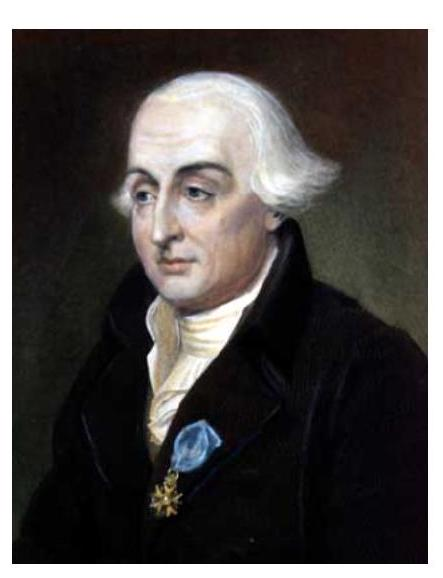
\includegraphics[max width=\textwidth, center]{2025_03_28_69fb641a049744196071g-09}
    Joseph Louis Lagrange
  \end{tcolorbox}
\end{minipage}

\begin{proposition}{}{}
La matrice associée à une application linéaire $f \in \mathcal{L}\left(\mathbb{K}^{m}, \mathbb{K}^{n}\right)$ est \hide{unique}.
\end{proposition}

\begin{demo}
Soit $f \in \mathcal{L}\left(\mathbb{R}^{m}, \mathbb{R}^{n}\right)$. On considère deux matrices $A=\left(a_{i, j}\right)$ et $B=\left(b_{i, j}\right)$ associées à $f$, c'est à dire que, pour tout $\left(x_{1}, x_{2}, \ldots, x_{m}\right) \in \mathbb{K}^{m}$,

$$
f\left(x_{1}, x_{2}, \ldots, x_{m}\right)=\left(\begin{array}{c}
a_{1,1} x_{1}+a_{1,2} x_{2}+\ldots+a_{1, m} x_{m} \\
a_{2,1} x_{1}+a_{2,2} x_{2}+\ldots+a_{2, m} x_{m} \\
\ldots \\
\ldots \\
a_{n, 1} x_{1}+a_{n, 2} x_{2}+\ldots+a_{n, m} x_{m}
\end{array}\right)=\left(\begin{array}{c}
b_{1,1} x_{1}+b_{1,2} x_{2}+\ldots+b_{1, m} x_{m} \\
b_{2,1} x_{1}+b_{2,2} x_{2}+\ldots+b_{2, m} x_{m} \\
\ldots \\
\ldots \\
b_{n, 1} x_{1}+b_{n, 2} x_{2}+\ldots+b_{n, m} x_{m}
\end{array}\right) .
$$

Pour $\left(x_{1}, \ldots, x_{n}\right)=(0, \ldots, 0,1,0, \ldots, 0)$, on voit que les coefficients $a_{i, j}$ et $b_{i, j}$ de la colonne correspondante à la position du 1 sont égaux. Par suite, on en déduit que, pour tous $i$ et pour tous $j, a_{i, j}=b_{i, j}$.\\
Cela signifie que $A=B$.
\end{demo}

\newpage

\subsection{Définition du produit de matrices}
\begin{remark}
On considère deux applications linéaires $f$ et $g$ de $\mathbb{K}^{3}$ dans $\mathbb{K}^{3}$ avec $\operatorname{Mat}(f)=\left(\begin{array}{lll}a_{1,1} & a_{1,2} & a_{1,3} \\ a_{2,1} & a_{2,2} & a_{2,3} \\ a_{3,1} & a_{3,2} & a_{3,3}\end{array}\right)$ et $\operatorname{Mat}(g)=\left(\begin{array}{lll}b_{1,1} & b_{1,2} & b_{1,3} \\ b_{2,1} & b_{2,2} & b_{2,3} \\ b_{3,1} & b_{3,2} & b_{3,3}\end{array}\right)$. On souhaite déterminer $\operatorname{Mat}(f \circ g)$.\\
Pour tout $\left(x_{1}, x_{2}, x_{3}\right) \in \mathbb{K}^{3}$ :

$$
\begin{aligned}
& f \circ g\left(x_{1}, x_{2}, x_{3}\right) \\
= & f\left(g\left(x_{1}, x_{2}, x_{3}\right)\right) \\
= & f\left(\left(\begin{array}{l}
b_{1,1} x_{1}+b_{1,2} x_{2}+b_{1,3} x_{3} \\
b_{2,1} x_{1}+b_{2,2} x_{2}+b_{2,3} x_{3} \\
b_{3,1} x_{1}+b_{3,2} x_{2}+b_{3,3} x_{3}
\end{array}\right)\right) \\
= & \left(\begin{array}{l}
a_{1,1}\left(b_{1,1} x_{1}+b_{1,2} x_{2}+b_{1,3} x_{3}\right)+a_{1,2}\left(b_{2,1} x_{1}+b_{2,2} x_{2}+b_{2,3} x_{3}\right)+a_{1,3}\left(b_{3,1} x_{1}+b_{3,2} x_{2}+b_{3,3} x_{3}\right) \\
a_{2,1}\left(b_{1,1} x_{1}+b_{1,2} x_{2}+b_{1,3} x_{3}\right)+a_{2,2}\left(b_{2,1} x_{1}+b_{2,2} x_{2}+b_{2,3} x_{3}\right)+a_{2,3}\left(b_{3,1} x_{1}+b_{3,2} x_{2}+b_{3,3} x_{3}\right) \\
a_{3,1}\left(b_{1,1} x_{1}+b_{1,2} x_{2}+b_{1,3} x_{3}\right)+a_{3,2}\left(b_{2,1} x_{1}+b_{2,2} x_{2}+b_{2,3} x_{3}\right)+a_{3,3}\left(b_{3,1} x_{1}+b_{3,2} x_{2}+b_{3,3} x_{3}\right)
\end{array}\right) \\
= & \left(\begin{array}{l}
\left(a_{1,1} b_{1,1}+a_{1,2} b_{2,1}+a_{1,3} b_{3,1}\right) x_{1}+\left(a_{1,1} b_{1,2}+a_{1,2} b_{2,2}+a_{1,3} b_{3,2}\right) x_{2}+\left(a_{1,1} b_{1,3}+a_{1,2} b_{2,3}+a_{1,3} b_{3,3}\right) x_{3} \\
\left(a_{2,1} b_{1,1}+a_{2,2} b_{2,1}+a_{2,3} b_{3,1}\right) x_{1}+\left(a_{2,1} b_{1,2}+a_{2,2} b_{2,2}+a_{2,3} b_{3,2}\right) x_{2}+\left(a_{2,1} b_{1,3}+a_{2,2} b_{2,3}+a_{2,3} b_{3,3}\right) x_{3} \\
\left(a_{3,1} b_{1,1}+a_{3,2} b_{2,1}+a_{3,3} b_{3,1}\right) x_{1}+\left(a_{3,1} b_{1,2}+a_{3,2} b_{2,2}+a_{3,3} b_{3,2}\right) x_{2}+\left(a_{3,1} b_{1,3}+a_{3,2} b_{2,3}+a_{3,3} b_{3,3}\right) x_{3}
\end{array}\right)
\end{aligned}
$$

Ainsi, on voit que

$$
\operatorname{Mat}(f \circ g)=\left(\begin{array}{lll}
a_{1,1} b_{1,1}+a_{1,2} b_{2,1}+a_{1,3} b_{3,1} & a_{1,1} b_{1,2}+a_{1,2} b_{2,2}+a_{1,3} b_{3,2} & a_{1,1} b_{1,3}+a_{1,2} b_{2,3}+a_{1,3} b_{3,3} \\
a_{2,1} b_{1,1}+a_{2,2} b_{2,1}+a_{2,3} b_{3,1} & a_{2,1} b_{1,2}+a_{2,2} b_{2,2}+a_{2,3} b_{3,2} & a_{2,1} b_{1,3}+a_{2,2} b_{2,3}+a_{2,3} b_{3,3} \\
a_{3,1} b_{1,1}+a_{3,2} b_{2,1}+a_{3,3} b_{3,1} & a_{3,1} b_{1,2}+a_{3,2} b_{2,2}+a_{3,3} b_{3,2} & a_{3,1} b_{1,3}+a_{3,2} b_{2,3}+a_{3,3} b_{3,3}
\end{array}\right)
$$
\end{remark}

La remarque précédente nous mène à définir le produit de deux matrices de la façon suivante :

\begin{definition}{}{}
Si A est une matrice de taille $n \times p$ et B une matrice de taille $p \times m$, le \textbf{produit des matrices $\mathbf{A}$ et $\mathbf{B}$}, noté $\mathrm{A} \times \mathrm{B}$ ou AB , est la matrice $\mathrm{C}=\left(c_{i, j}\right)$ de taille $n \times m$ telle que, pour tous $1 \leqslant i \leqslant n$ et $1 \leqslant j \leqslant m$, on a :

$$
c_{i, j}=\sum_{k=1}^{p} \hideM{a_{i, k} b_{k, j}}
$$
\end{definition}

\begin{center}
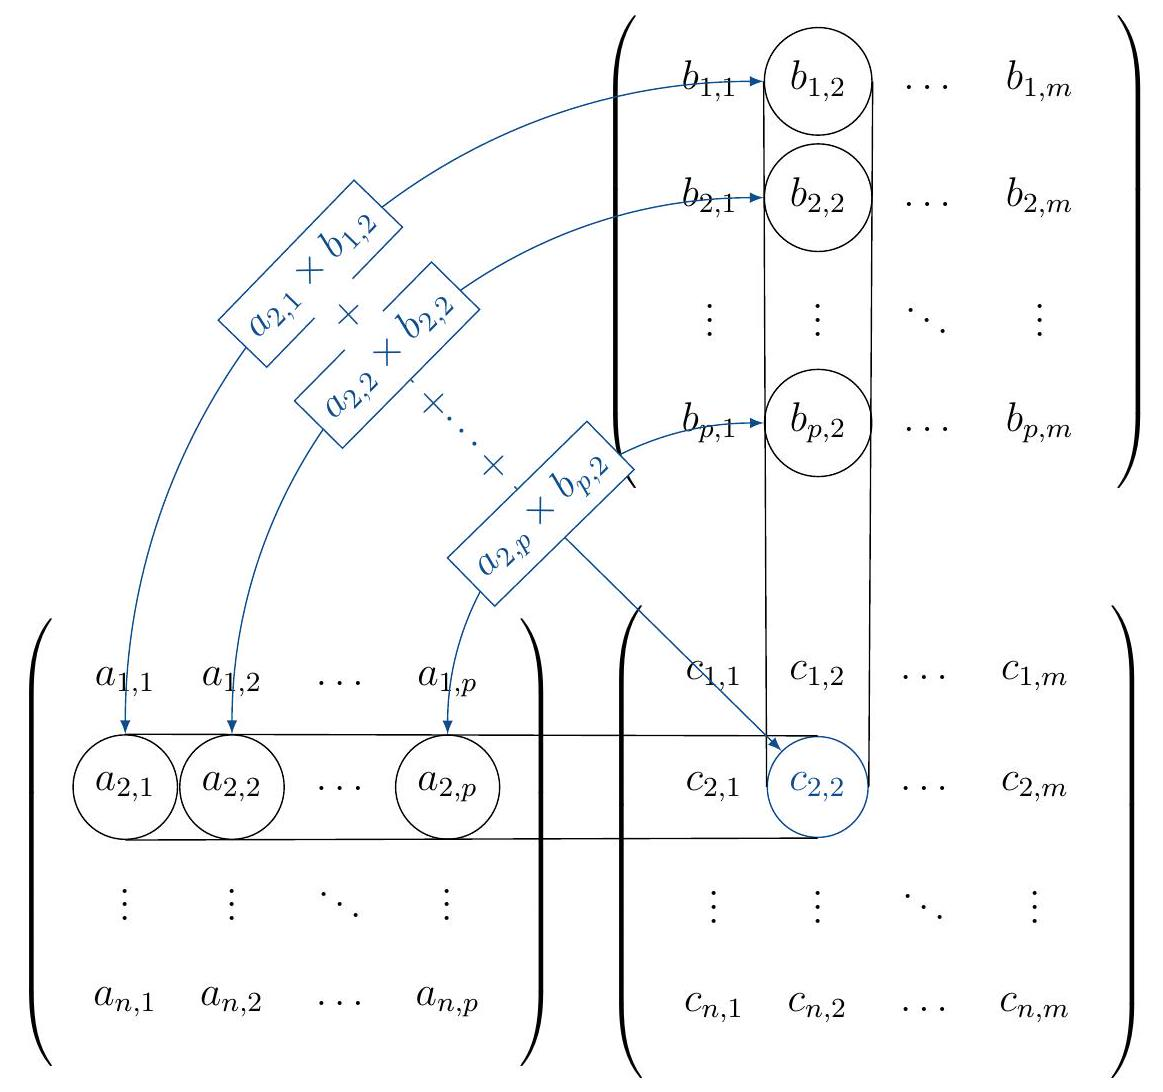
\includegraphics[width=0.8\textwidth]{2025_03_28_69fb641a049744196071g-11}
\end{center}

\begin{proposition}{}{}
Soient $f: \mathbb{K}^{p} \longrightarrow \mathbb{K}^{n}$ et $g: \mathbb{K}^{m} \longrightarrow \mathbb{K}^{p}$ deux applications linéaires. On a alors

$$
\operatorname{Mat}(f \circ g)=\hideM{\operatorname{Mat}(f) \times \operatorname{Mat}(g)}
$$
\end{proposition}

\begin{demo}
Dans le cas où $n=m=3$, cela découle directement de la remarque précédente.
\end{demo}

\subsection{Propriétés du produit de matrices}
\begin{proposition}{(admise)}
Soient $\mathrm{A}, \mathrm{B}$ et C trois matrices et $\lambda \in \mathbb{K}$. Sous réserve de définition des produit et des sommes, on a :

\begin{itemize}[noitemsep,topsep=0pt]
  \item $(\mathrm{A} \times \mathrm{B}) \times \mathrm{C}=\mathrm{A} \times(\mathrm{B} \times \mathrm{C})$\qquad (\textbf{associativité})
  \item $A \times(B+C)=A \times B+A \times C$\qquad (\textbf{distributivité à gauche})
  \item $(\mathrm{A}+\mathrm{B}) \times \mathrm{C}=\mathrm{A} \times \mathrm{C}+\mathrm{B} \times \mathrm{C}$\qquad (\textbf{distributivité à droite})
  \item $(\lambda \mathrm{A}) \times \mathrm{B}=\mathrm{A} \times(\lambda \mathrm{B})=\lambda(\mathrm{A} \times \mathrm{B})$. (\textbf{compatibilité avec le produit par un scalaire})
  \item $I_{n} \times \mathrm{A}=\mathrm{A} \times \mathrm{I}_{n}=\mathrm{A}$.\qquad ( $\mathrm{I}_{n}$ est l'\textbf{élément neutre} pour la multiplication de matrices)
\end{itemize}
\end{proposition}

\begin{remark}
Le produit matriciel n'est pas commutatif. On a en général, $\mathrm{A} \times \mathrm{B} \neq \mathrm{B} \times \mathrm{A}$.
\end{remark}

\begin{definition}{}{}
Soient A une matrice carrée $n$ et $k \in \mathbb{N}$.\\
La puissance $\mathbf{k}^{\mathbf{e}}$ de A, notée $\mathrm{A}^{k}$ est la matrice

$$
\mathrm{A}^{k}=\hideM{\underbrace{\mathrm{A} \times \mathrm{A} \times \ldots \times \mathrm{A}}_{k \text { facteurs }}} .
$$
\end{definition}

\begin{remark}
Si A est une matrice non nulle, $\mathrm{A}^{0}=\mathrm{I}_{n}$.
\end{remark}

\noindent
\begin{minipage}{.7\textwidth}
  \begin{history}{Opérations sur les matrices}{}
    En 1858, le mathématicien britannique Arthur Cayley (18211895) publie un article intitulé \emph{A memoir on the Theory of Matrices} dans lequel il définit les opérations usuelles du calcul matriciel (addition, multiplication, inversibilité) et montre les propriétés de distributivité et d'associativité. Il utilise en fait les matrices d'une façon abstraite et beaucoup plus générale que ce qui avait été fait avant lui.
  \end{history}
\end{minipage}
\hspace{1em}
\begin{minipage}{0.3\textwidth}
  \begin{tcolorbox}[colback=white,colframe=BrownHist]
    \centering
    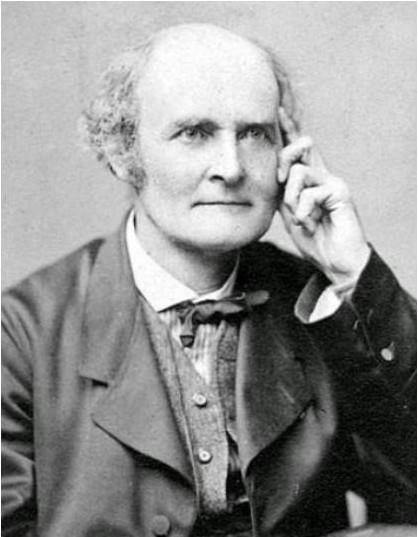
\includegraphics[max width=\textwidth, center]{2025_03_28_69fb641a049744196071g-12}
    Arthur Cayley
  \end{tcolorbox}
\end{minipage}

\section{Inverse de matrice et résolution de systèmes linéaires}
\subsection{Cadre général}
On considère le système de $n$ équations linéaires suivant, d'inconnues $x_{1}, x_{2}, \ldots, x_{n}$ :

$$
\left\{\begin{array}{c}
a_{1,1} x_{1}+a_{1,2} x_{2}+\ldots+a_{1, n} x_{n}=b_{1} \\
a_{2,1} x_{1}+a_{2,2} x_{2}+\ldots+a_{2, n} x_{n}=b_{2} \\
\ldots \\
\ldots \\
a_{n, 1} x_{1}+a_{n, 2} x_{2}+\ldots+a_{n, n} x_{n}=b_{n}
\end{array}\right.
$$

En posant $\mathrm{A}=\left(\begin{array}{cccc}a_{1,1} & a_{1,2} & \ldots & a_{1, n} \\ a_{2,1} & a_{2,2} & \ldots & a_{2, n} \\ \vdots & \vdots & \vdots & \vdots \\ a_{n, 1} & a_{n, 2} & \ldots & a_{n, n}\end{array}\right), \mathrm{X}=\left(\begin{array}{c}x_{1} \\ x_{2} \\ \vdots \\ x_{n}\end{array}\right)$, et $\mathrm{B}=\left(\begin{array}{c}b_{1} \\ b_{2} \\ \vdots \\ b_{n}\end{array}\right)$, on voit que le système précédent se réécrit de la manière suivante:

$$
\mathrm{AX}=\mathrm{B}
$$

\begin{definition}{}{}
Une matrice carrée A d'ordre $n$ est inversible lorsqu'il existe une matrice carrée B d'ordre $n$ telle que:

$$
\mathrm{A} \times \mathrm{B}=\hideM{\mathrm{B} \times \mathrm{A}=\mathrm{I}_{n}}
$$

La matrice $B$ est appelée l'\textbf{inverse} de la matrice $A$ et est notée $A^{-1}$.
\end{definition}

\begin{proposition}{}{}
En reprenant les notations précédents, si A est inversible, alors le système $\mathrm{A} X=\mathrm{B}$ admet une unique solution donnée par la matrice colonne $\mathrm{X}=\hideM{\mathrm{A}^{-1} \times \mathrm{B}}$.
\end{proposition}

\begin{demo}

$$
\begin{aligned}
\mathrm{AX}=\mathrm{B} & \Longleftrightarrow \mathrm{~A}^{-1} \times(\mathrm{AX})=\mathrm{A}^{-1} \times \mathrm{B} \\
& \Longleftrightarrow\left(\mathrm{~A}^{-1} \mathrm{~A}\right) \mathrm{X}=\mathrm{A}^{-1} \times \mathrm{B} \\
& \Longleftrightarrow \mathrm{I}_{n} \times \mathrm{X}=\mathrm{A}^{-1} \times \mathrm{B} \\
& \Longleftrightarrow \mathrm{X}=\mathrm{A}^{-1} \times \mathrm{B}
\end{aligned}
$$
\end{demo}

\subsection{Algorithme du pivot de Gauss}
Dans l'algorithme du pivot de Gauss, les opérations effectuées à chaque étape reviennent à multiplier la matrice du système (à gauche) par certaines matrices. Plus précisément :

\begin{itemize}[noitemsep,topsep=0pt]
  \item Multiplier la ie ligne par un scalaire non nul $\lambda$ revient à multiplier le système par la matrice suivante (\textbf{matrice de dilatation}) :

$$
\left(\begin{array}{ccccc}
1 & 0 & \ldots & \ldots & 0 \\
0 & 1 & \ddots & & \vdots \\
\vdots & \ddots & \lambda & \ddots & \vdots \\
\vdots & & \ddots & 1 & 0 \\
0 & \ldots & \ldots & 0 & 1
\end{array}\right)
$$

  \item Échanger la ligne i et la ligne j revient à multiplier le système par la matrice suivante (\textbf{matrice de permutation}) :

$$
\left(\begin{array}{cccccc}
1 & 0 & \ldots & \ldots & \ldots & 0 \\
0 & 1 & \ddots & & & \vdots \\
\vdots & \ddots & 0 & \ddots & 1 & \vdots \\
\vdots & & \ddots & 1 & \ddots & \vdots \\
\vdots & & 1 & \ddots & 0 & 0 \\
0 & \ldots & \ldots & \ldots & 0 & 1
\end{array}\right)
$$

  \item Ajouter $\lambda \times$ Ligne i à la ligne j revient à multiplier le système par la matrice suivante (\textbf{matrice de transvection})

$$
\left(\begin{array}{cccccc}
1 & 0 & \ldots & \ldots & \ldots & 0 \\
0 & 1 & \ddots & & & \vdots \\
\vdots & \ddots & 1 & \ddots & & \vdots \\
\vdots & & \ddots & 1 & \ddots & \vdots \\
\vdots & \lambda & & \ddots & 1 & 0 \\
0 & \ldots & \ldots & \ldots & 0 & 1
\end{array}\right)
$$
\end{itemize}

\begin{definition}{}{}
L'ensemble des matrices de dilatation, de permutation et de transvection sont appelées matrices élémentaires.
\end{definition}

\begin{proposition}{}{}
Toute matrice élémentaire est inversible. Par ailleurs, l'inverse d'une matrice élémentaire est une matrice élémentaire.
\end{proposition}

\begin{demo}
\begin{itemize}[noitemsep,topsep=0pt]
  \item L'opération inverse d'une dilatation de rapport $\lambda$ est une dilation de rapport $\frac{1}{\lambda}$. On en déduit qu'une matrice de dilatation est inversible et que son inverse est une matrice de dilatation.
  \item L'opération inverse d'une permutation est cette permutation elle même. On en déduit qu'une matrice de permutation est inversible et qu'elle est égale à son inverse (elle vérifie $\mathrm{A}=\mathrm{A}^{-1}$)
  \item L'opération inverse de la transvection $L_{j} \leftarrow L_{j}+\lambda L_{i}$ est la transvection $L_{j} \leftarrow L_{j}-\lambda L_{i}$. On en déduit qu'une matrice de transvection est inversible et que son inverse est une matrice de transvection.
\end{itemize}
\end{demo}

\begin{proposition}{}{}
Soit A une matrice carrée d'ordre $n$ et inversible. Il existe des matrices élémentaires $\mathrm{P}_{1}, \mathrm{P}_{2}, \ldots, \mathrm{P}_{k}$ telles que $\mathrm{P}_{k} \times \ldots \times \mathrm{P}_{2} \times \mathrm{P}_{1} \times \mathrm{A}=\hideM{\mathrm{I}_{n}}$.\\
On a alors $\mathrm{A}^{-1}=\hideM{\mathrm{P}_{k} \times \ldots \times \mathrm{P}_{2} \times \mathrm{P}_{1}}$.
\end{proposition}

\begin{demo}
On applique les différentes étapes du pivot de Gauss à la matrice $A$ afin d'obtenir une matrice de la forme suivante :

$$
M=\left(\begin{array}{cccccc}
* & \diamond & \ldots & \ldots & \ldots & \diamond \\
0 & * & \ddots & & & \vdots \\
\vdots & \ddots & * & \ddots & & \vdots \\
\vdots & & \ddots & * & \ddots & \vdots \\
\vdots & & & \ddots & * & \diamond \\
0 & \ldots & \ldots & \ldots & 0 & *
\end{array}\right)
$$

Chaque coefficient représenté par une étoile sera en fait non nul étant donné que A est inversible et que le système correspondant admet une unique solution.\\
Par des dilations successives, il est donc possible d'obtenir des 1 sur la diagonale. On utilise ensuite des transvections afin de faire apparaître des 0 sur les coefficients strictement au dessus de la diagonale. Finalement, on obtient bien la matrice $I_{n}$.\\
Comme le fait d'effectuer des permutations, des dilatations et des transvections revient exactement à multiplier la matrice A à gauche par des matrices élémentaires, on en déduit qu'il existe bien des matrices élémentaires $\mathrm{P}_{i}$ telles que $\mathrm{I}_{n}=\mathrm{P}_{k} \times \ldots \times \mathrm{P}_{2} \times \mathrm{P}_{1} \times \mathrm{A}$.
\end{demo}

\begin{remark}
\begin{itemize}
  \item[]
  \item Si A n'est pas inversible, la matrice obtenue par le pivot de Gauss dans la démonstration précédente aura nécessairement un coefficient nul sur la diagonale.
  \item Si A est inversible, comme $A^{-1}=P_{k} \times \ldots \times P_{2} \times P_{1}=P_{k} \times \ldots \times P_{2} \times P_{1} \times \mathrm{I}_{n}$, on voit que si l'on part de la matrice identité et que l'on effectue les permutations, dilatations et transvections correspondant aux matrices $\mathrm{P}_{i}$, on obtient la matrice $\mathrm{A}^{-1}$.
\end{itemize}
\end{remark}

\begin{method}{Déterminer l'inverse d'une matrice (lorsque l'inverse existe)}{}
\begin{itemize}[noitemsep,topsep=0pt]
  \item On effectue l'algorithme du pivot de Gauss afin d'obtenir la matrice $I_{n}$ (si après avoir effectué l'algorithme du pivot, certains coefficients de la diagonale sont nuls, la matrice n'est pas inversible).
  \item Pour obtenir l'inverse de la matrice, il suffit d'appliquer les mêmes opérations dans le même ordre à la matrice $\mathrm{I}_{n}$.
\end{itemize}
\end{method}

\begin{example}
Montrer que la matrice $A=\left(\begin{array}{ll}2 & 3 \\ 1 & 5\end{array}\right)$ est inversible est déterminer $A^{-1}$.\\
Solution :\\
On effectue l'algorithme du pivot de Gauss :\\
$\left(\begin{array}{ll}2 & 3 \\ 1 & 5\end{array}\right) \underset{L_{1} \leftrightarrow L_{2}}{\longrightarrow}\left(\begin{array}{ll}1 & 5 \\ 2 & 3\end{array}\right) \underset{L_{2} \leftarrow L_{2}-2 L_{1}}{\longrightarrow}\left(\begin{array}{cc}1 & 5 \\ 0 & -7\end{array}\right) \underset{L_{2} \leftarrow-\frac{1}{7} L_{2}}{\longrightarrow}\left(\begin{array}{ll}1 & 5 \\ 0 & 1\end{array}\right) \underset{L_{1} \leftarrow L_{1}-5 L_{2}}{\longrightarrow}\left(\begin{array}{ll}1 & 0 \\ 0 & 1\end{array}\right)$.\\
On effectue alors les mêmes opérations à la matrice $I_{2}$ :\\
$\left(\begin{array}{ll}1 & 0 \\ 0 & 1\end{array}\right) \underset{L_{1} \leftrightarrow L_{2}}{\longrightarrow}\left(\begin{array}{ll}0 & 1 \\ 1 & 0\end{array}\right) \underset{L_{2} \leftarrow L_{2}-2 L_{1}}{\longrightarrow}\left(\begin{array}{cc}0 & 1 \\ 1 & -2\end{array}\right) \underset{L_{2} \leftarrow-\frac{1}{7} L_{2}}{\longrightarrow}\left(\begin{array}{cc}0 & 1 \\ -\frac{1}{7} & \frac{2}{7}\end{array}\right) \underset{L_{1} \leftarrow L_{1}-5 L_{2}}{\longrightarrow}\left(\begin{array}{cc}\frac{5}{7} & -\frac{3}{7} \\ -\frac{1}{7} & \frac{2}{7}\end{array}\right)
\\=A^{-1}$.
\end{example}

\subsection{Cas particulier des matrices de taille 2}
\begin{definition}{}{}
Soit $\mathrm{A}=\left(\begin{array}{ll}a & b \\ c & d\end{array}\right)$ une matrice carrée d'ordre 2.\\
Le \textbf{déterminant} de A est le nombre noté $\operatorname{det}(\mathrm{A})$ et défini par :

$$
\operatorname{det}(\mathrm{A})=\hideM{a d-b c}
$$
\end{definition}

\begin{proposition}{}{}
Une matrice carrée est inversible si, et seulement si, son déterminant est non nul. en particulier, si $\mathrm{A}=\left(\begin{array}{ll}a & b \\ c & d\end{array}\right)$ est inversible, $\mathrm{A}^{-1}=\dfrac{1}{\operatorname{det}(\mathrm{A})}\left(\hideM{\begin{array}{cc}d & -b \\ -c & a\end{array}}\right)$.
\end{proposition}

\begin{demo}
Soit $\mathrm{A}=\left(\begin{array}{ll}a & b \\ c & d\end{array}\right)$. On pose $\mathrm{B}=\left(\begin{array}{cc}d & -b \\ -c & a\end{array}\right)$.\\
On calcule $\mathrm{A} \times \mathrm{B}$ :

$$
\mathrm{A} \times \mathrm{B}=\left(\begin{array}{cc}
a d-b c & 0 \\
0 & a d-b c
\end{array}\right)
$$

\begin{itemize}[noitemsep,topsep=0pt]
  \item Si $\operatorname{det}(\mathrm{A}) \neq 0$, alors $\mathrm{A} \times \dfrac{1}{\operatorname{det}(\mathrm{A})} \mathrm{B}=\dfrac{1}{\operatorname{det}(\mathrm{A})}\left(\begin{array}{cc}a d-b c & 0 \\ 0 & a d-b c\end{array}\right)=I_{2}$.
  \item Si $\operatorname{det}(\mathrm{A})=0$, on veut montrer que A n'est pas inversible.
\end{itemize}

On suppose par l'absurde que A est inversible.

$$
\begin{array}{ll} 
& \mathrm{A} \times \mathrm{B}=\left(\begin{array}{ll}
0 & 0 \\
0 & 0
\end{array}\right) \\
\text { donc } & \mathrm{A}^{-1} \times \mathrm{A} \times \mathrm{B}=\mathrm{A}^{-1} \times\left(\begin{array}{ll}
0 & 0 \\
0 & 0
\end{array}\right) \\
\text { donc } & \mathrm{B}=\left(\begin{array}{ll}
0 & 0 \\
0 & 0
\end{array}\right) \\
\text { donc } & \mathrm{A}=\left(\begin{array}{ll}
0 & 0 \\
0 & 0
\end{array}\right)
\end{array}
$$

Cela est impossible car on a supposé que A était inversible.
\end{demo}

\noindent
\begin{minipage}{.7\textwidth}
  \begin{history}{Origine du mot matrice}{}
    La notion de déterminant se généralise pour des matrices de taille supérieure. En fait, c'est même le calcul de déterminants particuliers, appelés mineurs qui a inspiré le nom de «matrice» à son inventeur \textbf{James Joseph Sylvester} (1814-1897). Dans un article de 1851, il précise: «I have in previous papers defined a "Matrix" as a rectangular array of terms, out of which different systems of determinants may be engendered as from the womb of a common parent.» C'est ainsi qu'un terme dont l'origine étymologique se rapporte à la mère (du latin \emph{matricis}) a été employé pour désigner un tableau de nombres.
  \end{history}
\end{minipage}
\hspace{1em}
\begin{minipage}{0.35\textwidth}
  \begin{tcolorbox}[colback=white,colframe=BrownHist]
    \centering
    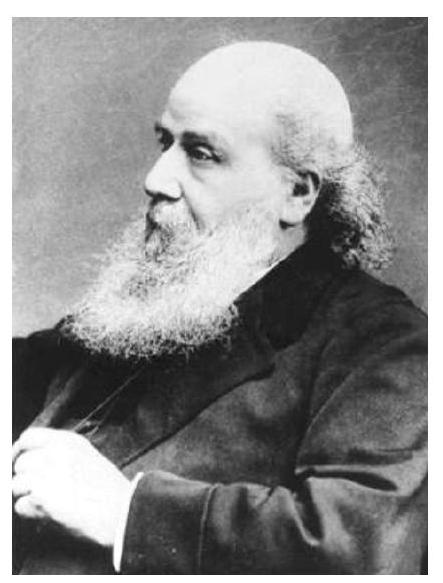
\includegraphics[max width=\textwidth, center]{2025_03_28_69fb641a049744196071g-16}
    James Joseph Sylvester
  \end{tcolorbox}
\end{minipage}

\begin{savoir}{}{}
\begin{itemize}[noitemsep,topsep=0pt]
  \item Calculer des sommes, des produits et des puissances de matrices.
  \item Déterminer, s'il existe, l'inverse d'une matrice à l'aide du pivot de Gauss.
  \item Utiliser le calcul matriciel pour résoudre un système linéaire.
  \item Modéliser une situation par une matrice.
\end{itemize}
\end{savoir}

\end{document}